\documentclass{beamer}

\mode<presentation> {

% The Beamer class comes with a number of default slide themes
% which change the colors and layouts of slides. Below this is a list
% of all the themes, uncomment each in turn to see what they look like.

%\usetheme{default}
%\usetheme{AnnArbor}
%\usetheme{Antibes}
%\usetheme{Bergen}
%\usetheme{Berkeley}
%\usetheme{Berlin}
%\usetheme{Boadilla}
%\usetheme{CambridgeUS}
%\usetheme{Copenhagen}
%\usetheme{Darmstadt}
%\usetheme{Dresden}
%\usetheme{Frankfurt}
%\usetheme{Goettingen}
%\usetheme{Hannover}
%\usetheme{Ilmenau}
%\usetheme{JuanLesPins}
%\usetheme{Luebeck}
\usetheme{Madrid}
%\usetheme{Malmoe}
%\usetheme{Marburg}
%\usetheme{Montpellier}
%\usetheme{PaloAlto}
%\usetheme{Pittsburgh}
%\usetheme{Rochester}
%\usetheme{Singapore}
%\usetheme{Szeged}
%\usetheme{Warsaw}

% As well as themes, the Beamer class has a number of color themes
% for any slide theme. Uncomment each of these in turn to see how it
% changes the colors of your current slide theme.

%\usecolortheme{albatross}
%\usecolortheme{beaver}
%\usecolortheme{beetle}
%\usecolortheme{crane}
%\usecolortheme{dolphin}
%\usecolortheme{dove}
%\usecolortheme{fly}
%\usecolortheme{lily}
%\usecolortheme{orchid}
%\usecolortheme{rose}
%\usecolortheme{seagull}
%\usecolortheme{seahorse}
%\usecolortheme{whale}
%\usecolortheme{wolverine}

}

\usepackage{graphicx} % Allows including images
\usepackage{booktabs} % Allows the use of \toprule, \midrule and \bottomrule in tables
\usepackage{listings}
\usepackage{hyperref}


%----------------------------------------------------------------------------------------
%	TITLE PAGE
%----------------------------------------------------------------------------------------

\title[DDB with Celery and RabbitMQ]{Performance Tuning and Analysis of Celery  and RabbitMQ}

\author{Robin}
\date{\today}

\begin{document}

\begin{frame}
\titlepage 
\end{frame}

\begin{frame}
\frametitle{Agenda} 
\tableofcontents 
\end{frame}

\section{Test Environment}
\begin{frame}
\frametitle{DDB Environment}
\begin{itemize}
\item EC2
	\begin{itemize}
	\item 4 machines
	\item Each instance has 6TB EBS disk
	\item c3.4xlarge, 16 vCPU, 30GB Memory
	\item we test the DDB with 4 Nodes
	\end{itemize}
\item Production
	\begin{itemize}
	\item 4 machines
	\item Each instance has 4TB SSD disk
	\item 32 CPU and 64GB memory
	\end{itemize}	
\end{itemize}
\end{frame}

\begin{frame}
\frametitle{Celery and RabbitMQ}
\begin{itemize}
\item Three Liquid Web machines intnodeb, intnodec, and intmaster are used to support Celery and RabbitMQ
	\begin{itemize}
	\item the three machines have same hardware
	\item 1.60TB disk, 30GB memory, 8 cores
	\end{itemize}
\item intmaster host RabbitMQ and test Client
\item 100 celery workers are launched in both intnodeb and intnodec
\end{itemize}
\end{frame}

\begin{frame}
\frametitle{Test Cases}
\begin{itemize}
\item We construct 669 identical test cases for AH, PH, ACB, PCB, ATC, PTC and UATC. We triple the test cases (2007)
	\begin{itemize}
	\item Randomize: shuffle all the test cases, and equal divide them to n processes. For each process, we shuffle the assigned test cases, and then run 
	\item n is in (1, 2, 4, 8, 16, 32, 48)
	\item we run the test in intmaster by \textbf{"for n in 8 1 2 4 8 16 32 48; do time python rabbitmq\_mess.py \$n; done | \& tee log"}
	\end{itemize}	
\end{itemize}
\end{frame}

\begin{frame}
\frametitle{How do features are parallelized?}
\textbf{Divide and Conquer}: each request is partitioned into small computation units by \textit{one} input parameters, then crate a celery task for each unit, finally result of units are combined and returned to client.
\begin{itemize}
\item AH/PH: date range is partitioned into three parts if the days of the range is greater than 30 days or not in same month.
\item ACB/PCB: 155 countries are partitioned into 10 chunks.
\item ATC/PTC/UATC: partitioned by feed id, one feed one task.
\end{itemize}
\textbf{Pivot and Granularity of Parallelism}
\begin{itemize}
\item Pivot: parallelism pivot highlighted by nature computation structure of each features.
\item Granularity: some is from problem structure, more are based on experiments. 
	\begin{itemize}
		\item the best granularity of {app, pub} country breakdown is 8 or 16.
	\end{itemize}
\end{itemize}
\end{frame}

\begin{frame}
\begin{figure}
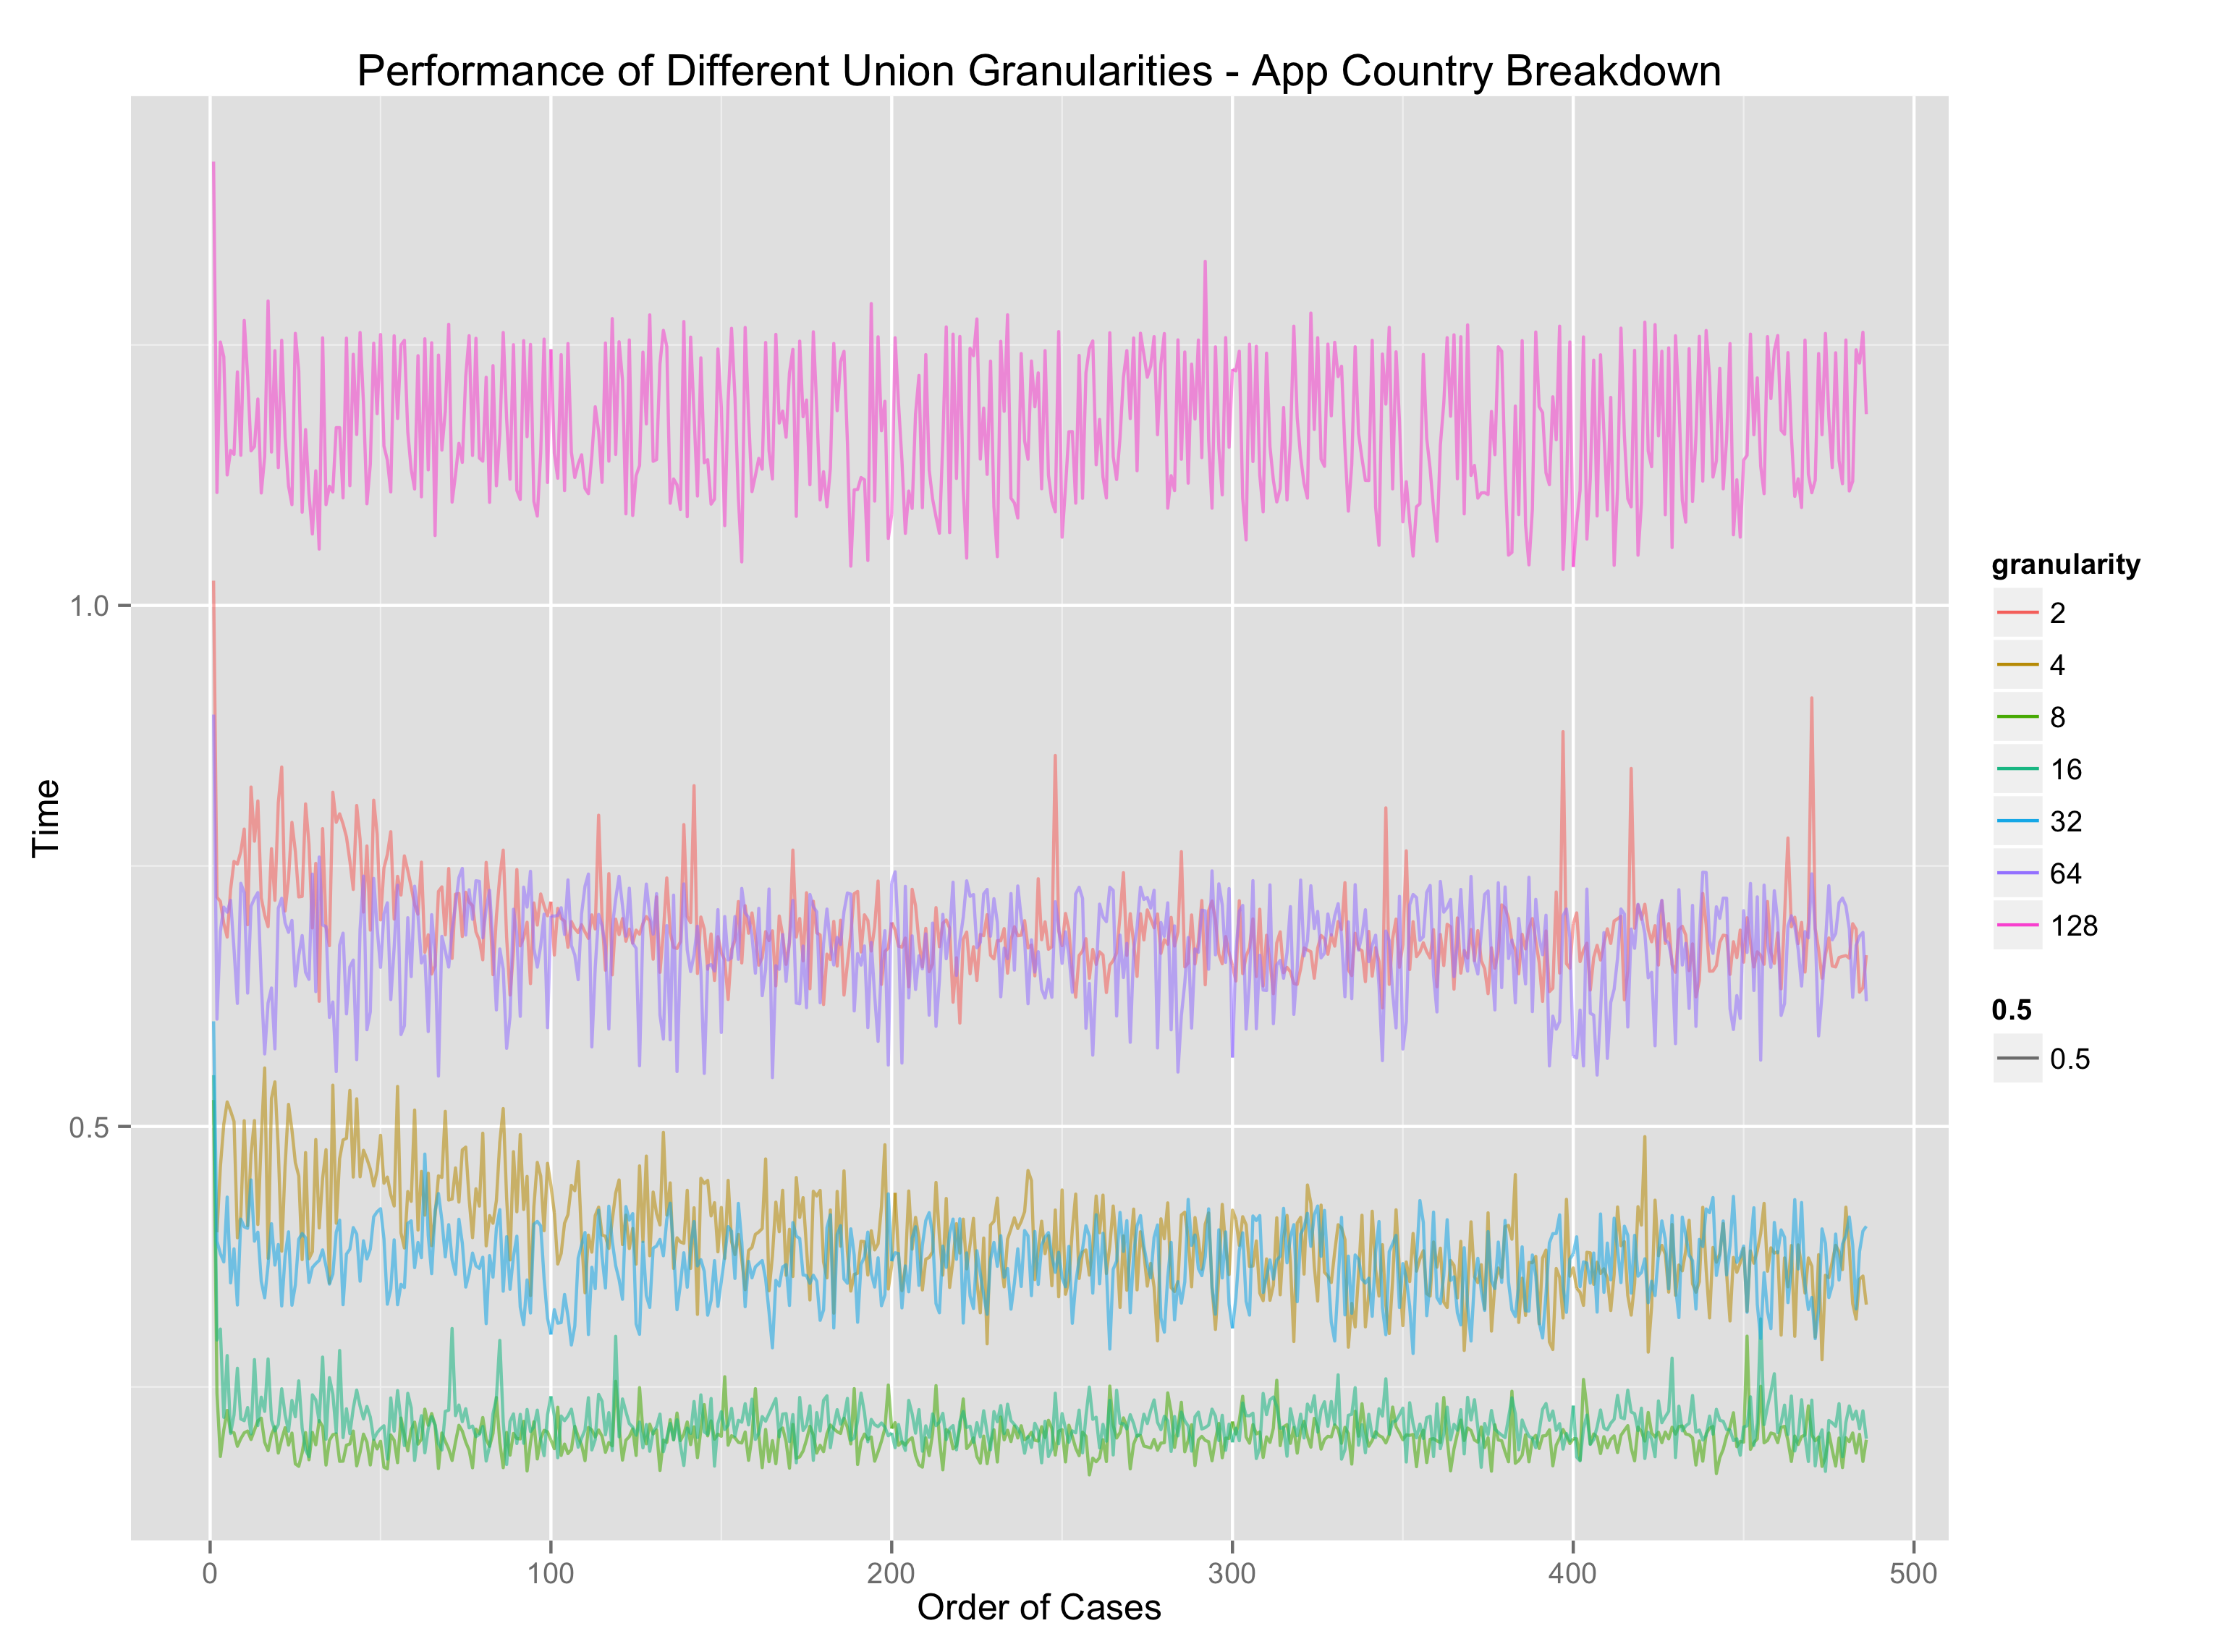
\includegraphics[width=\linewidth]{images/union_granularity.png}
\end{figure}
\end{frame}

\section{Performance Tuning}
\begin{frame}
\frametitle{Change configuration of Celery}
\begin{itemize}
\item librabbitmq
\item each individual task type has it's own rabbitmq queue
\item all queues are transient
\end{itemize}
\end{frame}

\section{Performance Analyze}

\begin{frame}
\begin{figure}
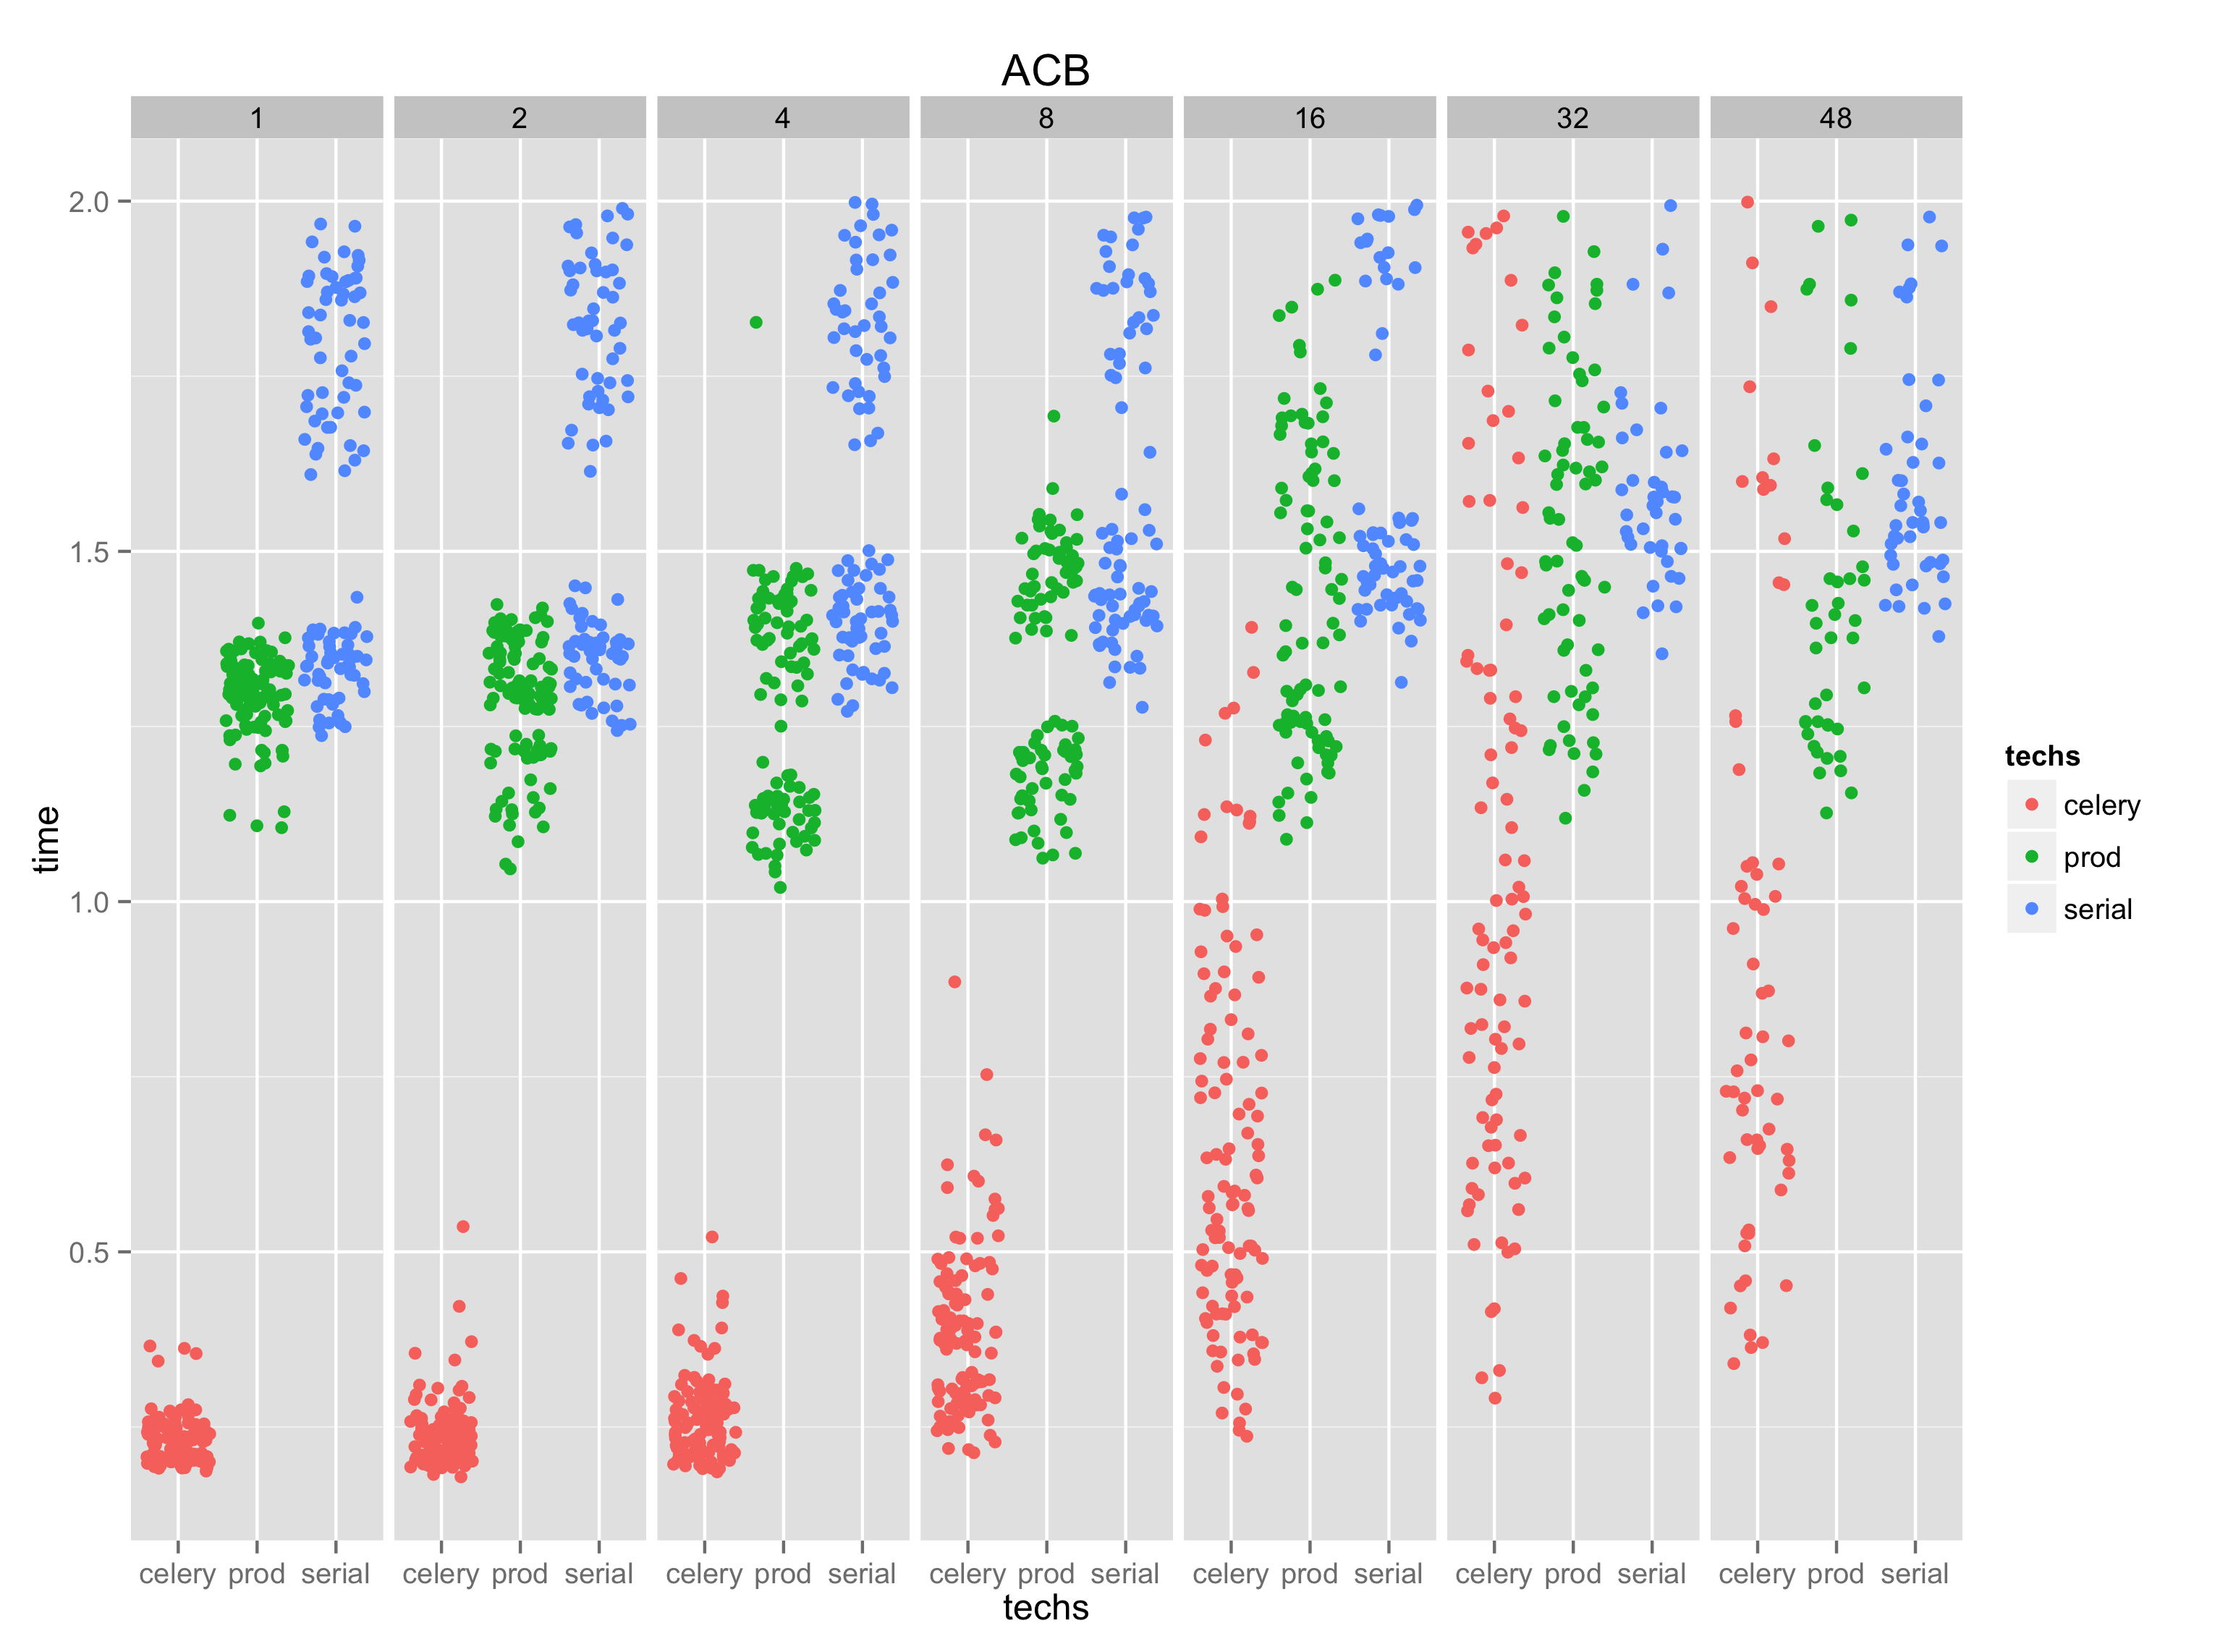
\includegraphics[width=\linewidth]{images/ACB.png}
\end{figure}

\end{frame}

\begin{frame}
\begin{figure}
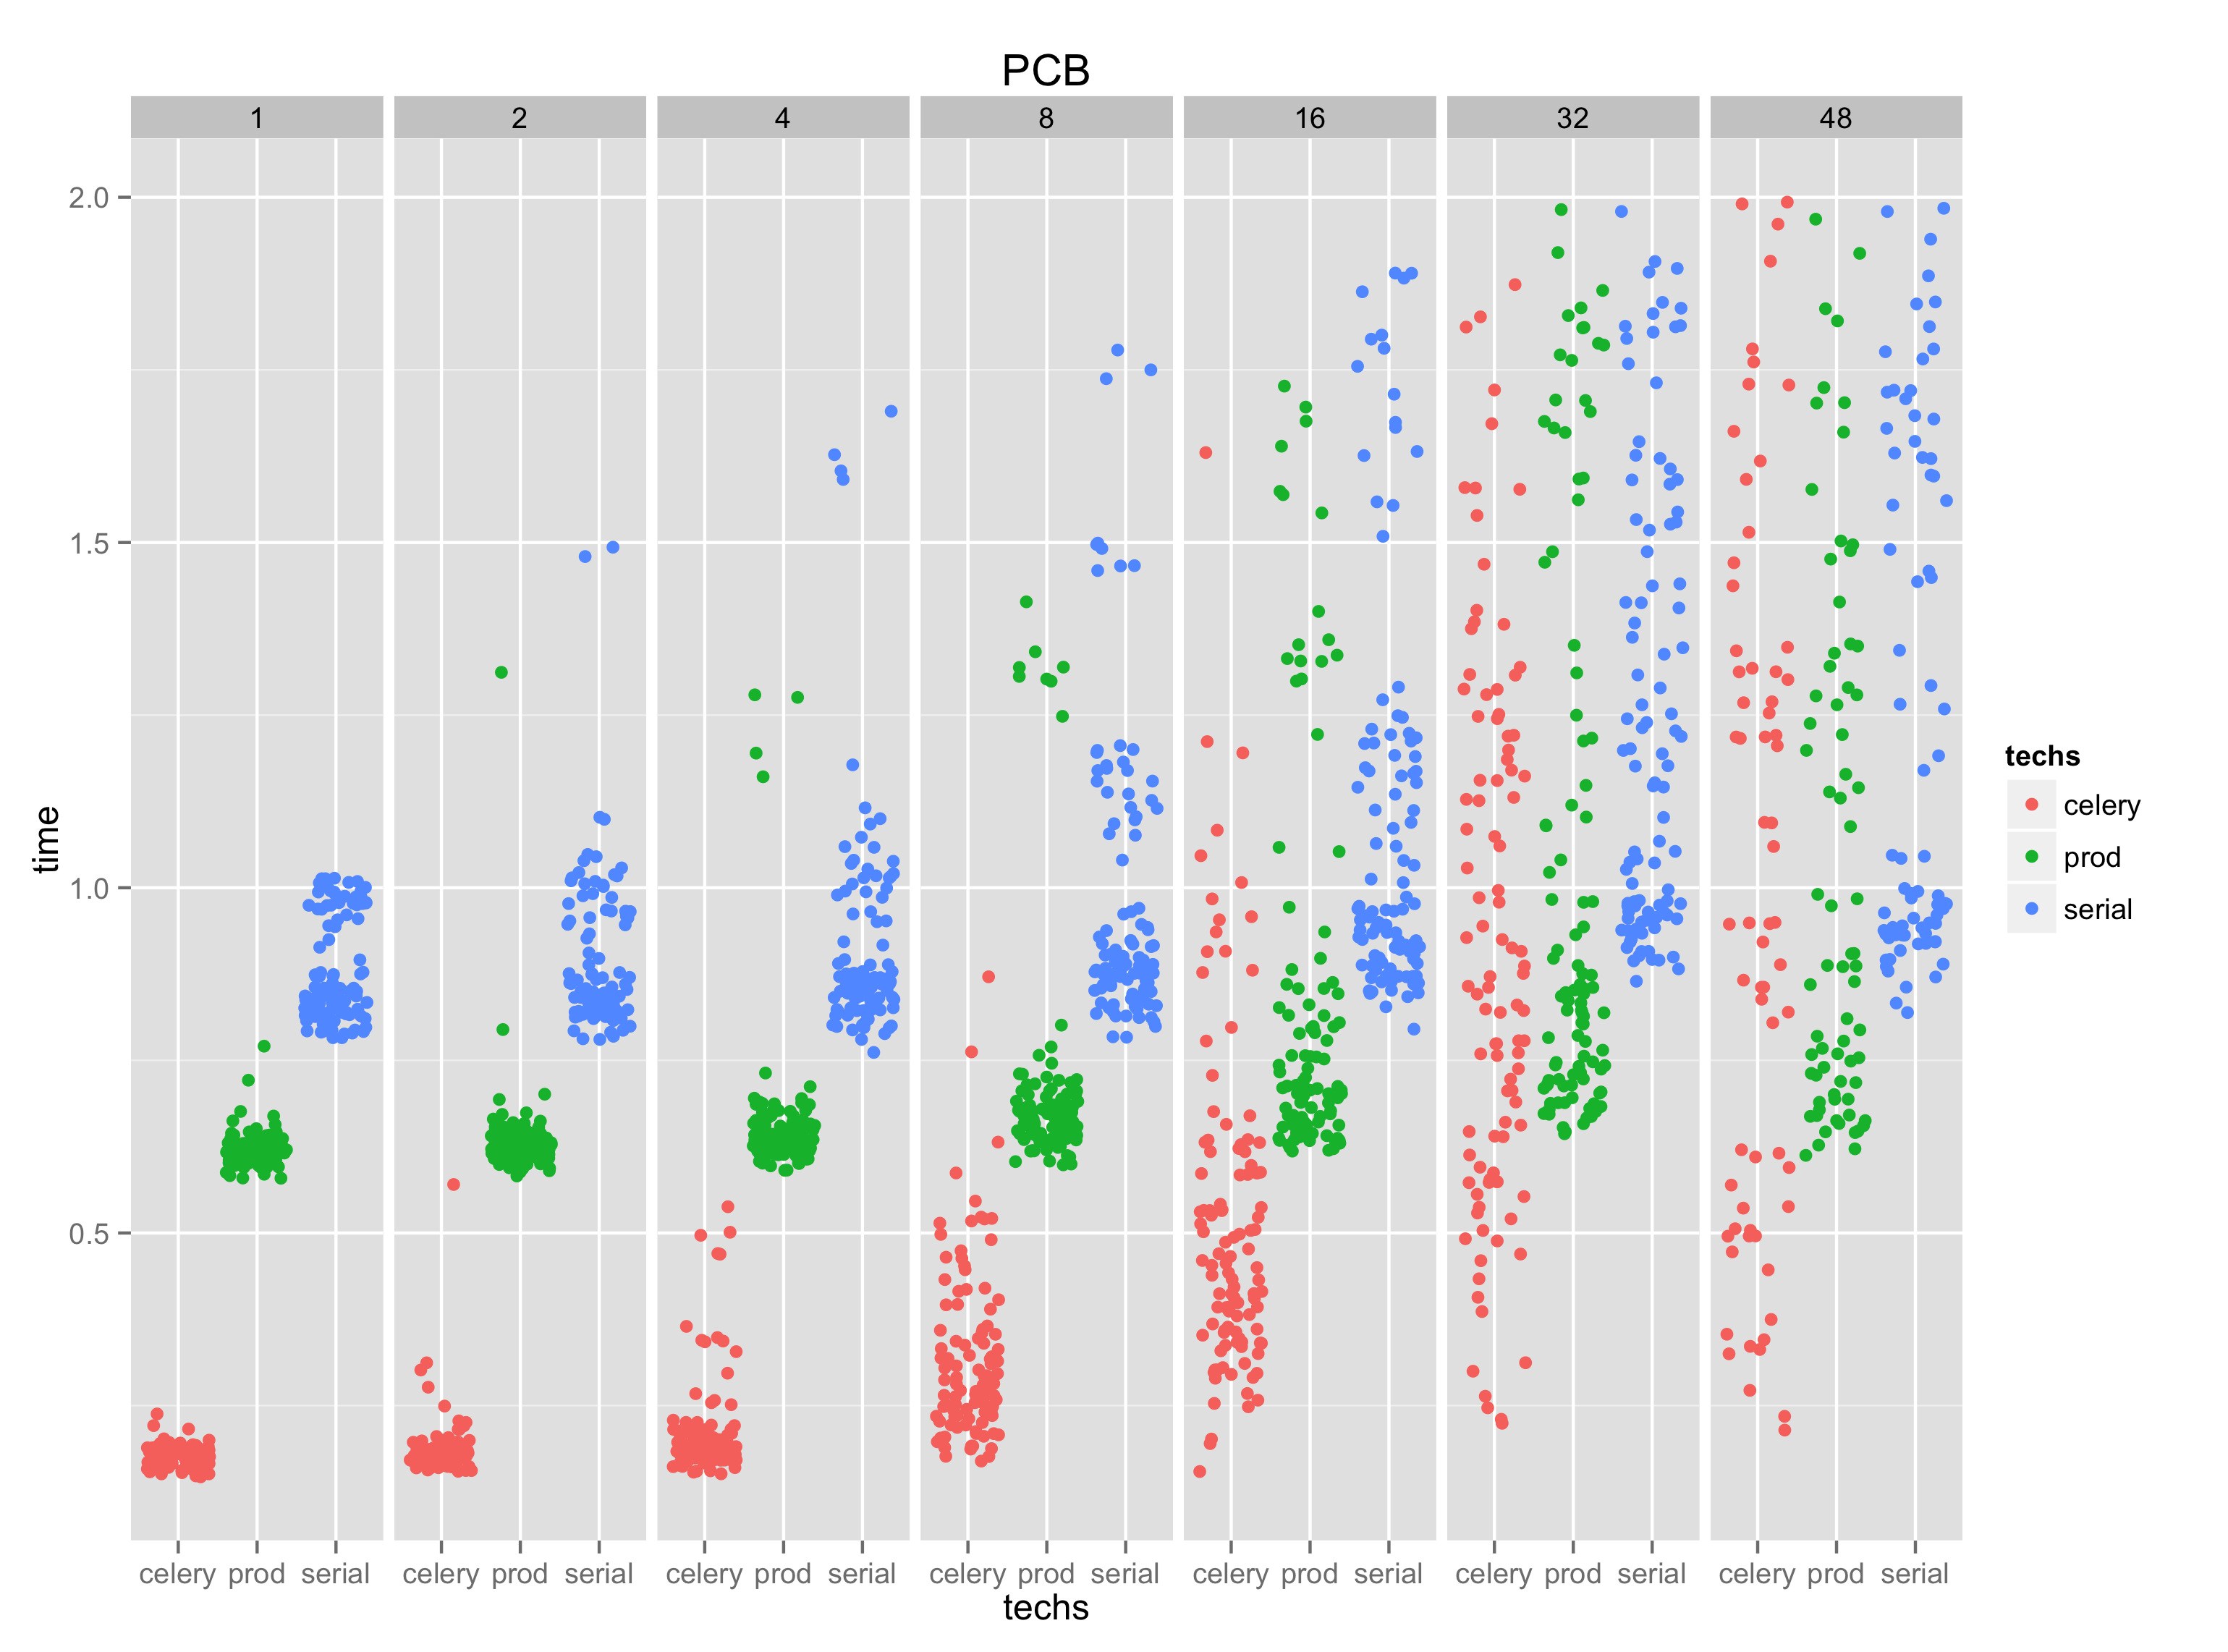
\includegraphics[width=\linewidth]{images/PCB.png}
\end{figure}
\end{frame}

\begin{frame}
\begin{figure}
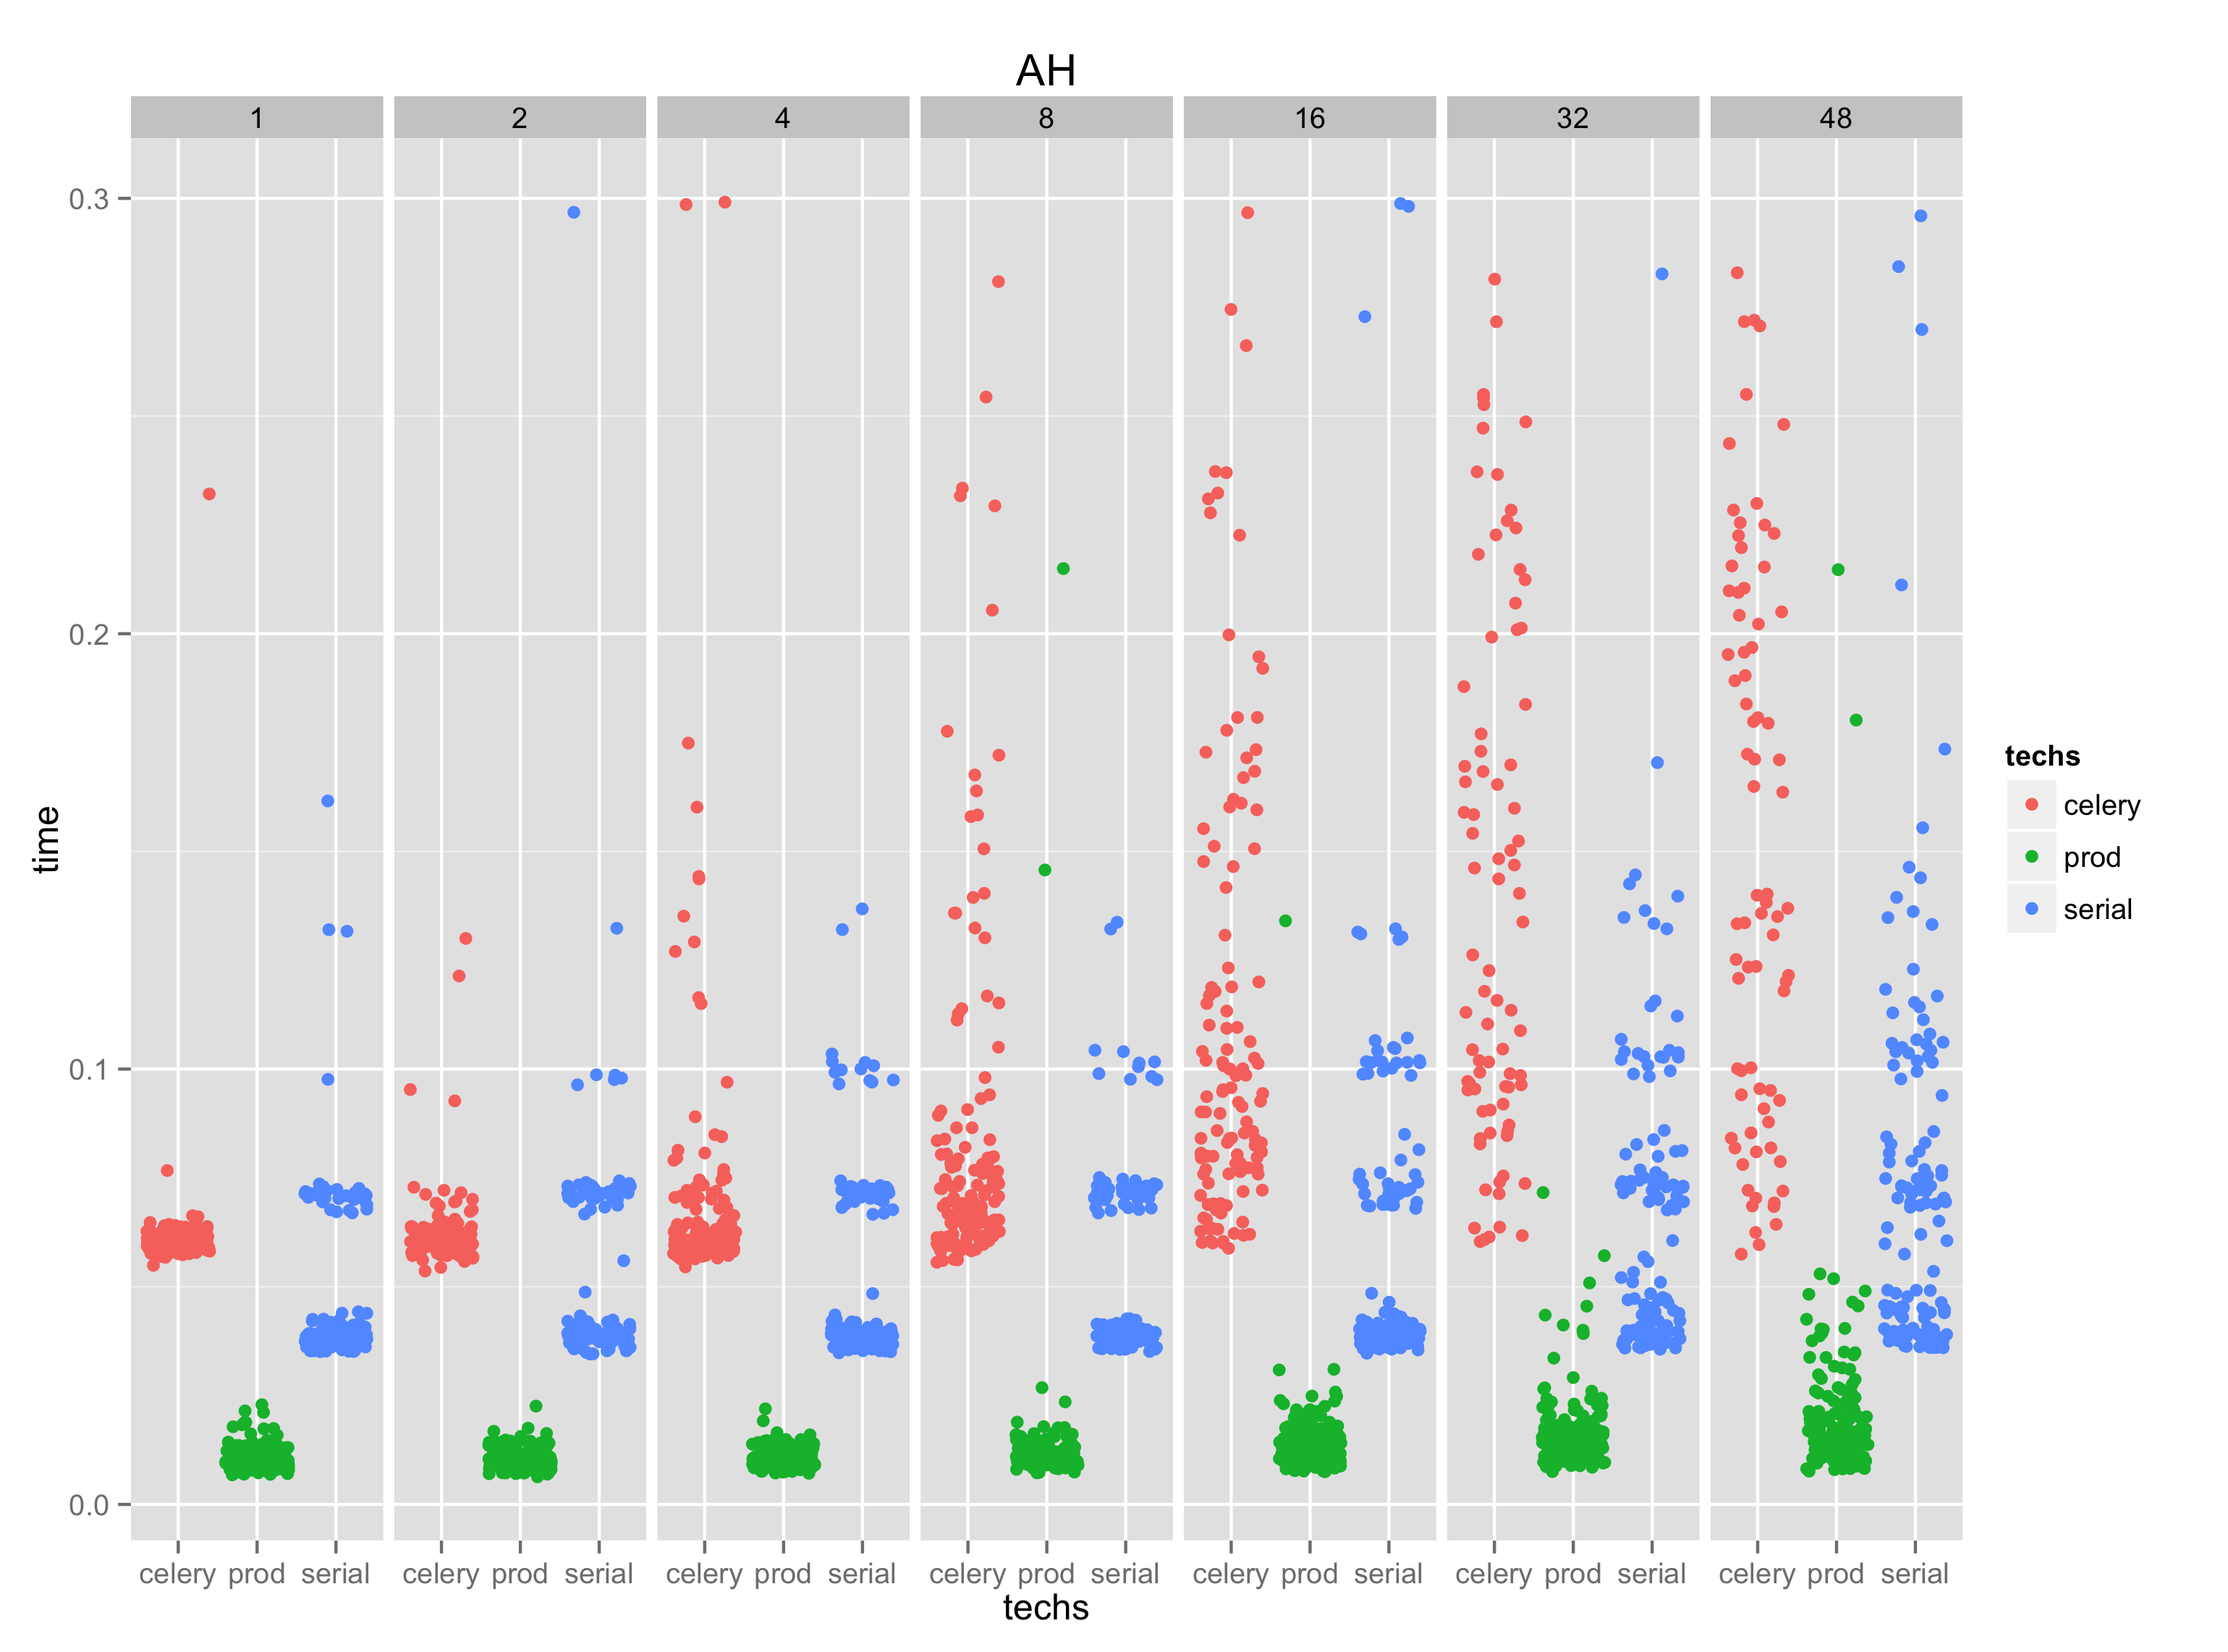
\includegraphics[width=\linewidth]{images/AH.png}
\end{figure}
\end{frame}

\begin{frame}
\begin{figure}
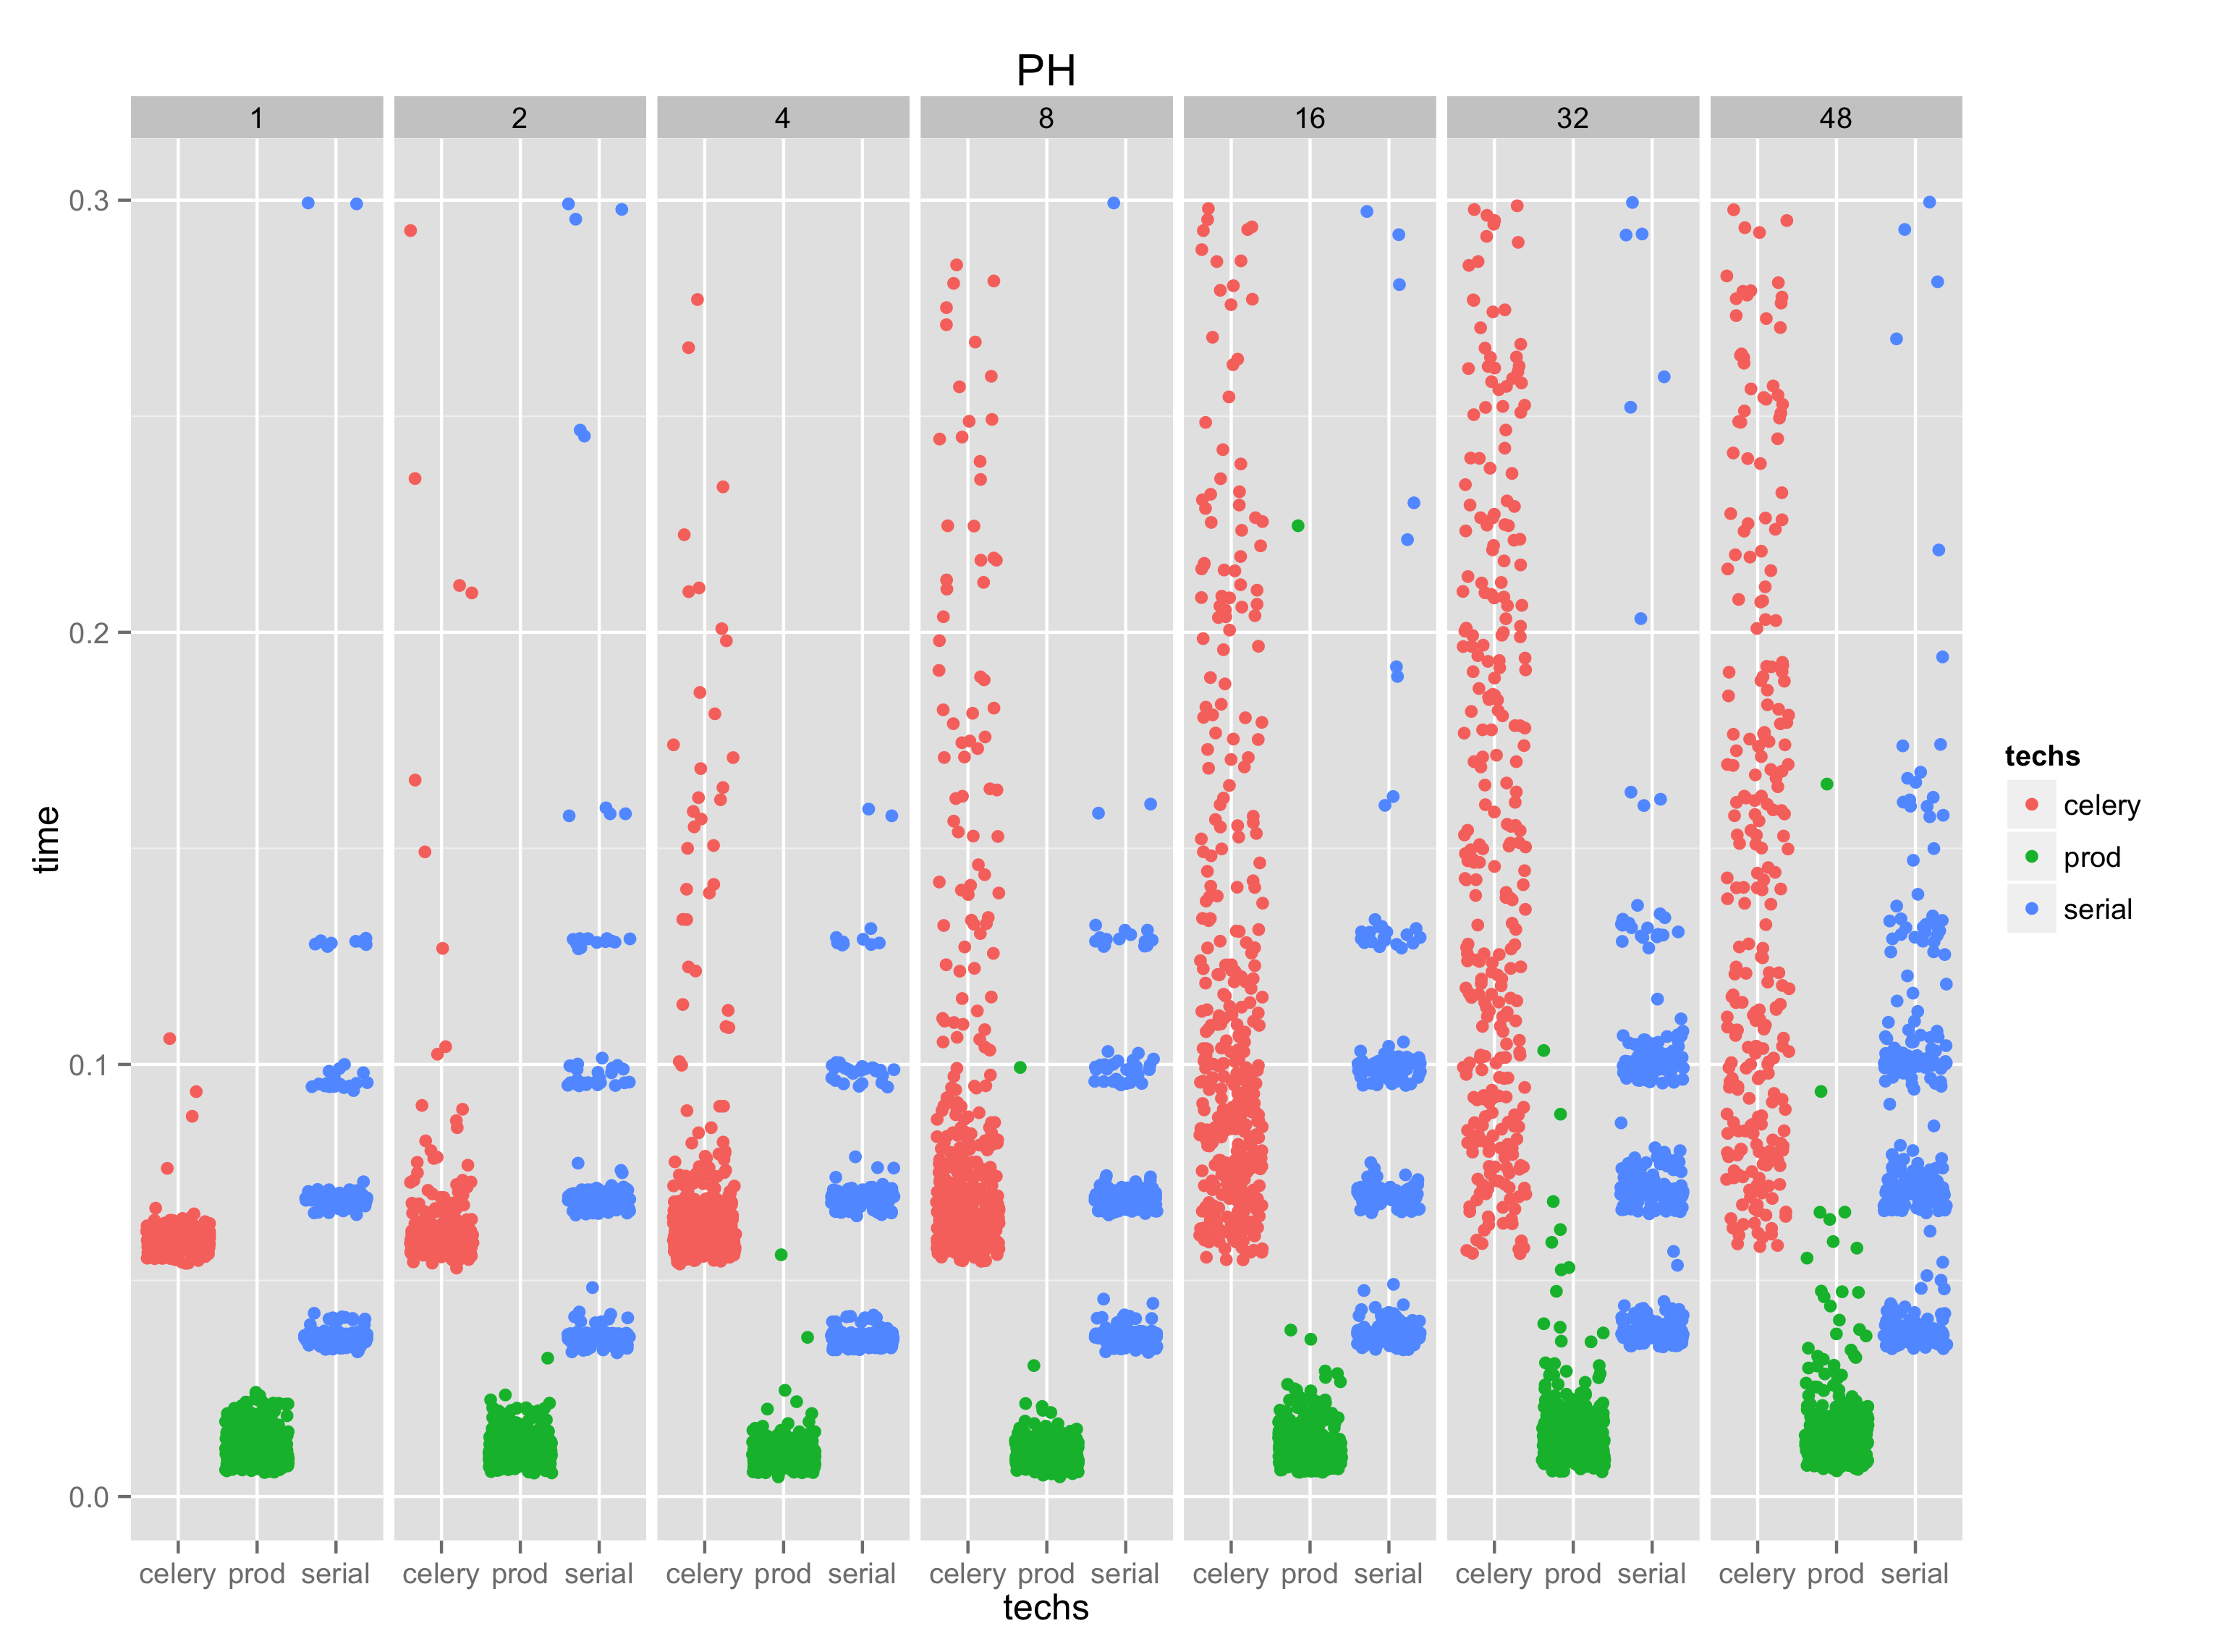
\includegraphics[width=\linewidth]{images/PH.png}
\end{figure}
\end{frame}

\begin{frame}
\begin{figure}
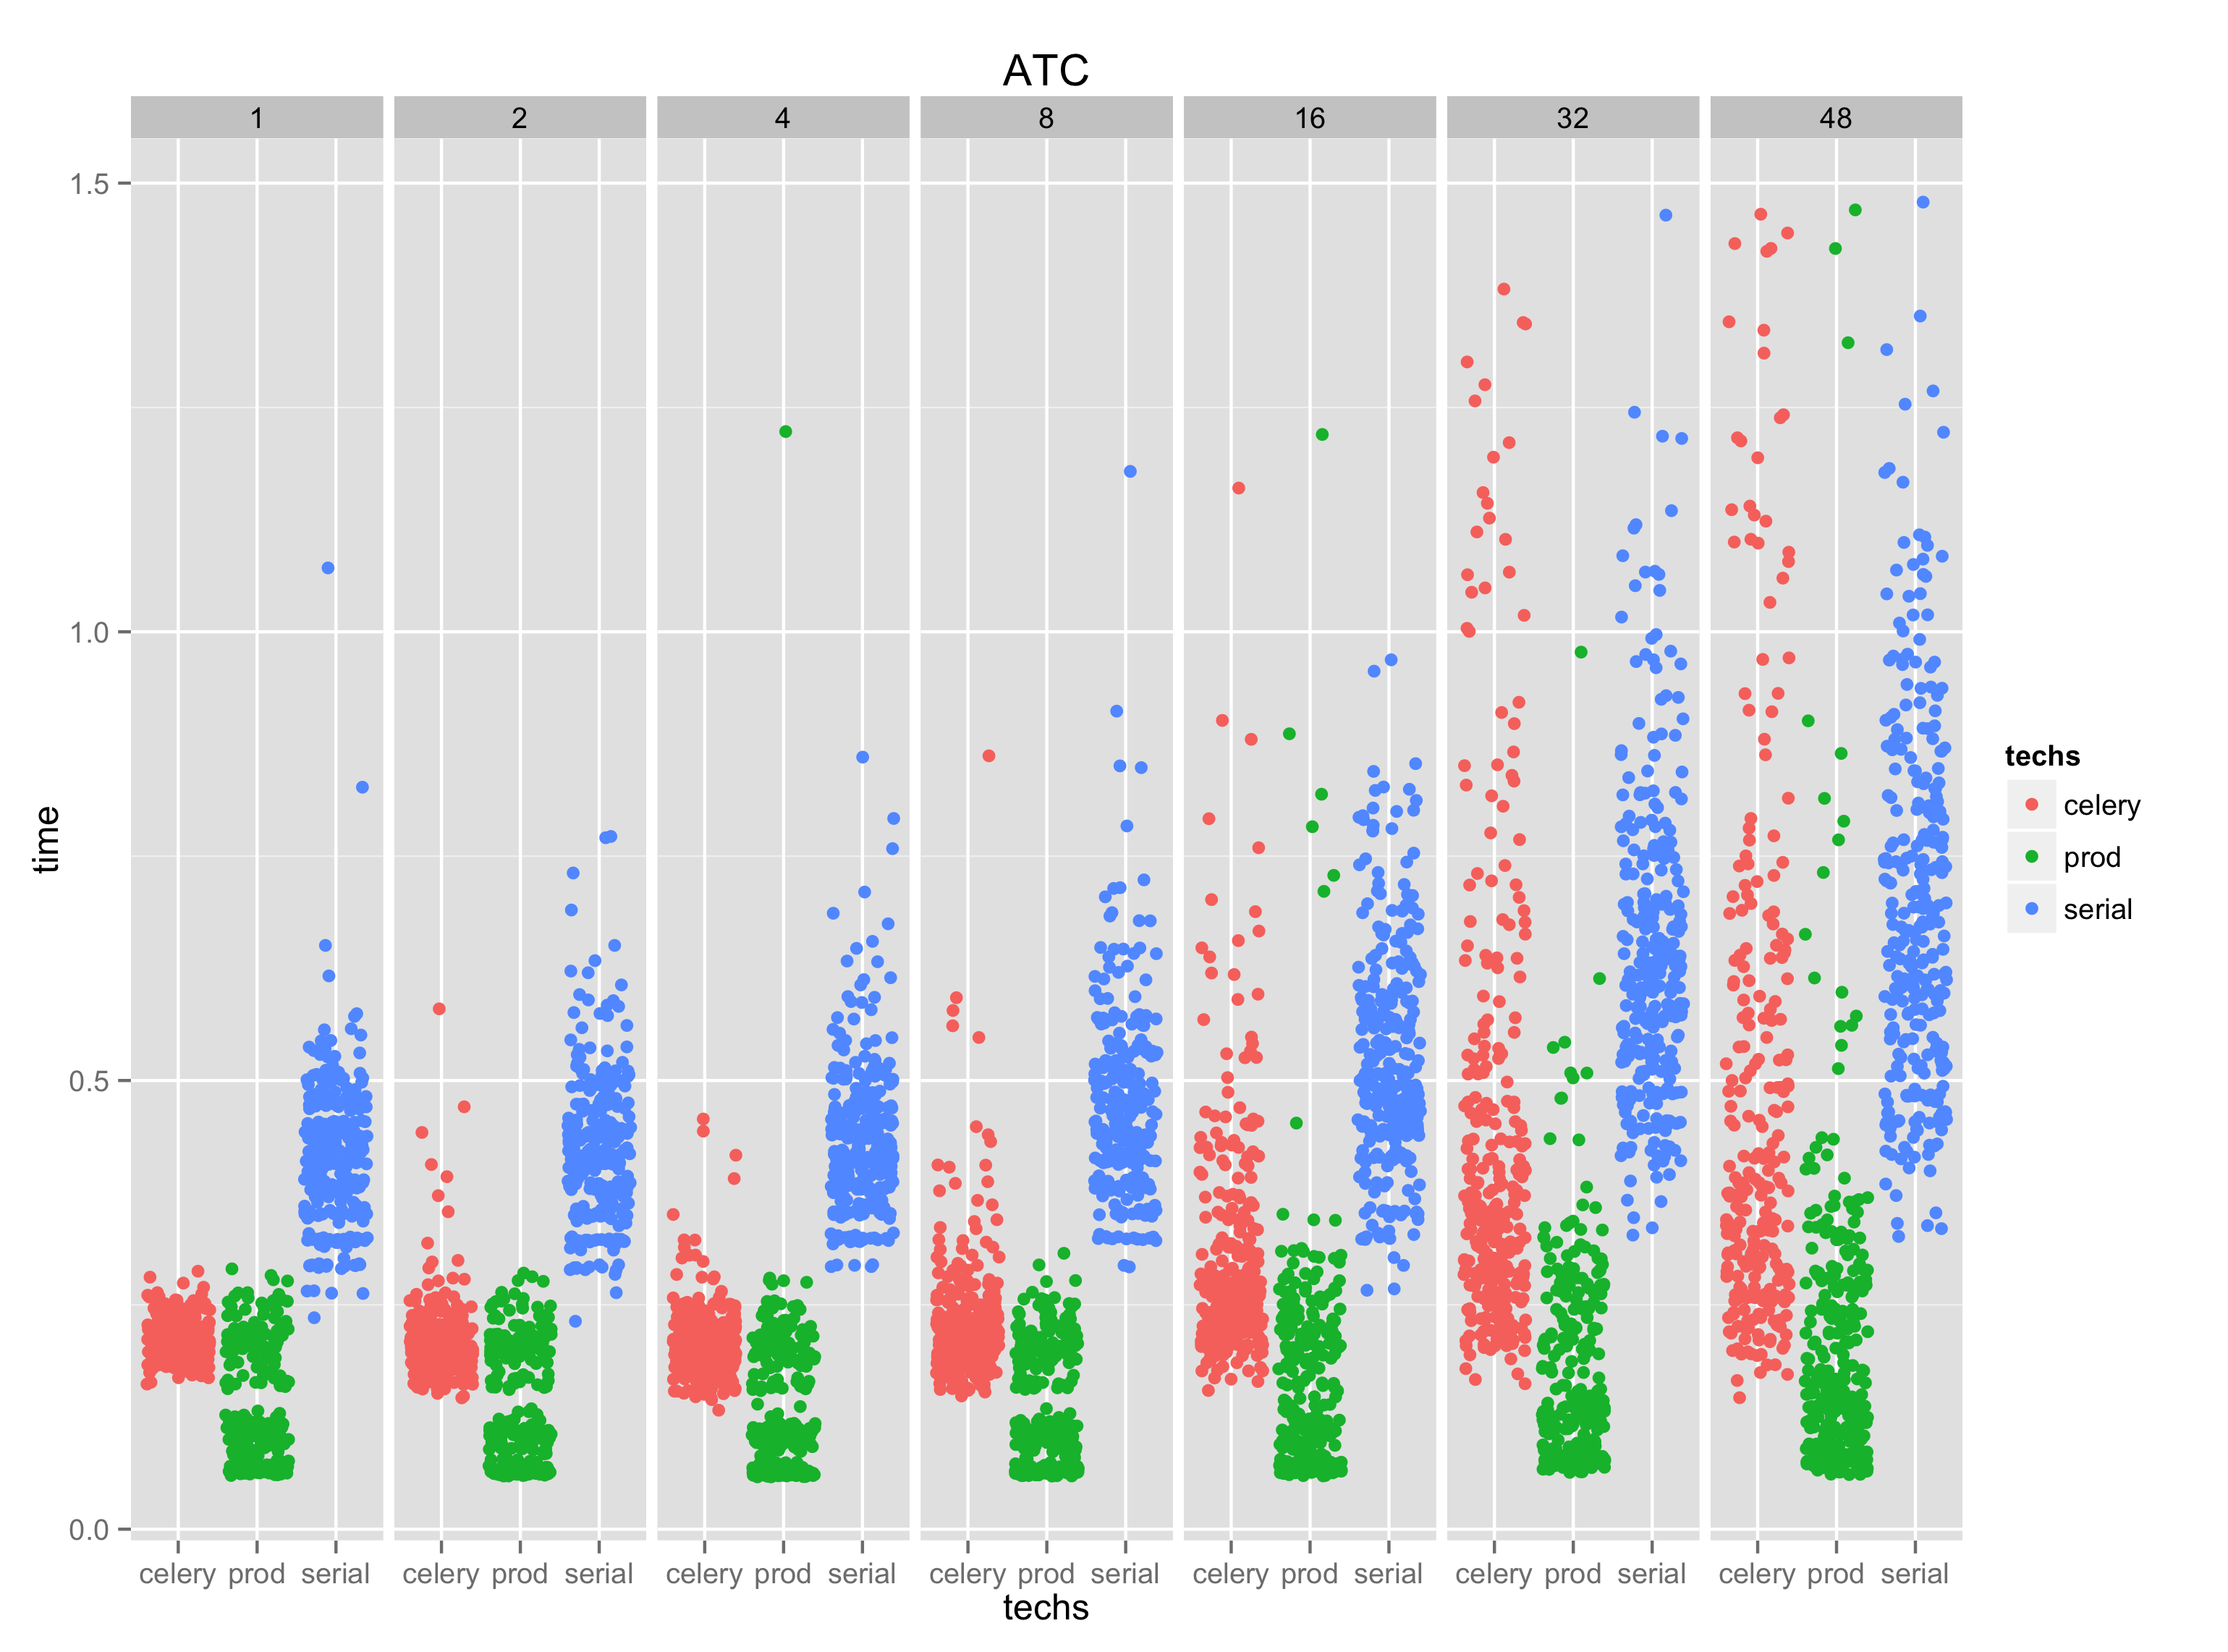
\includegraphics[width=\linewidth]{images/ATC.png}
\end{figure}
\end{frame}

\begin{frame}
\begin{figure}
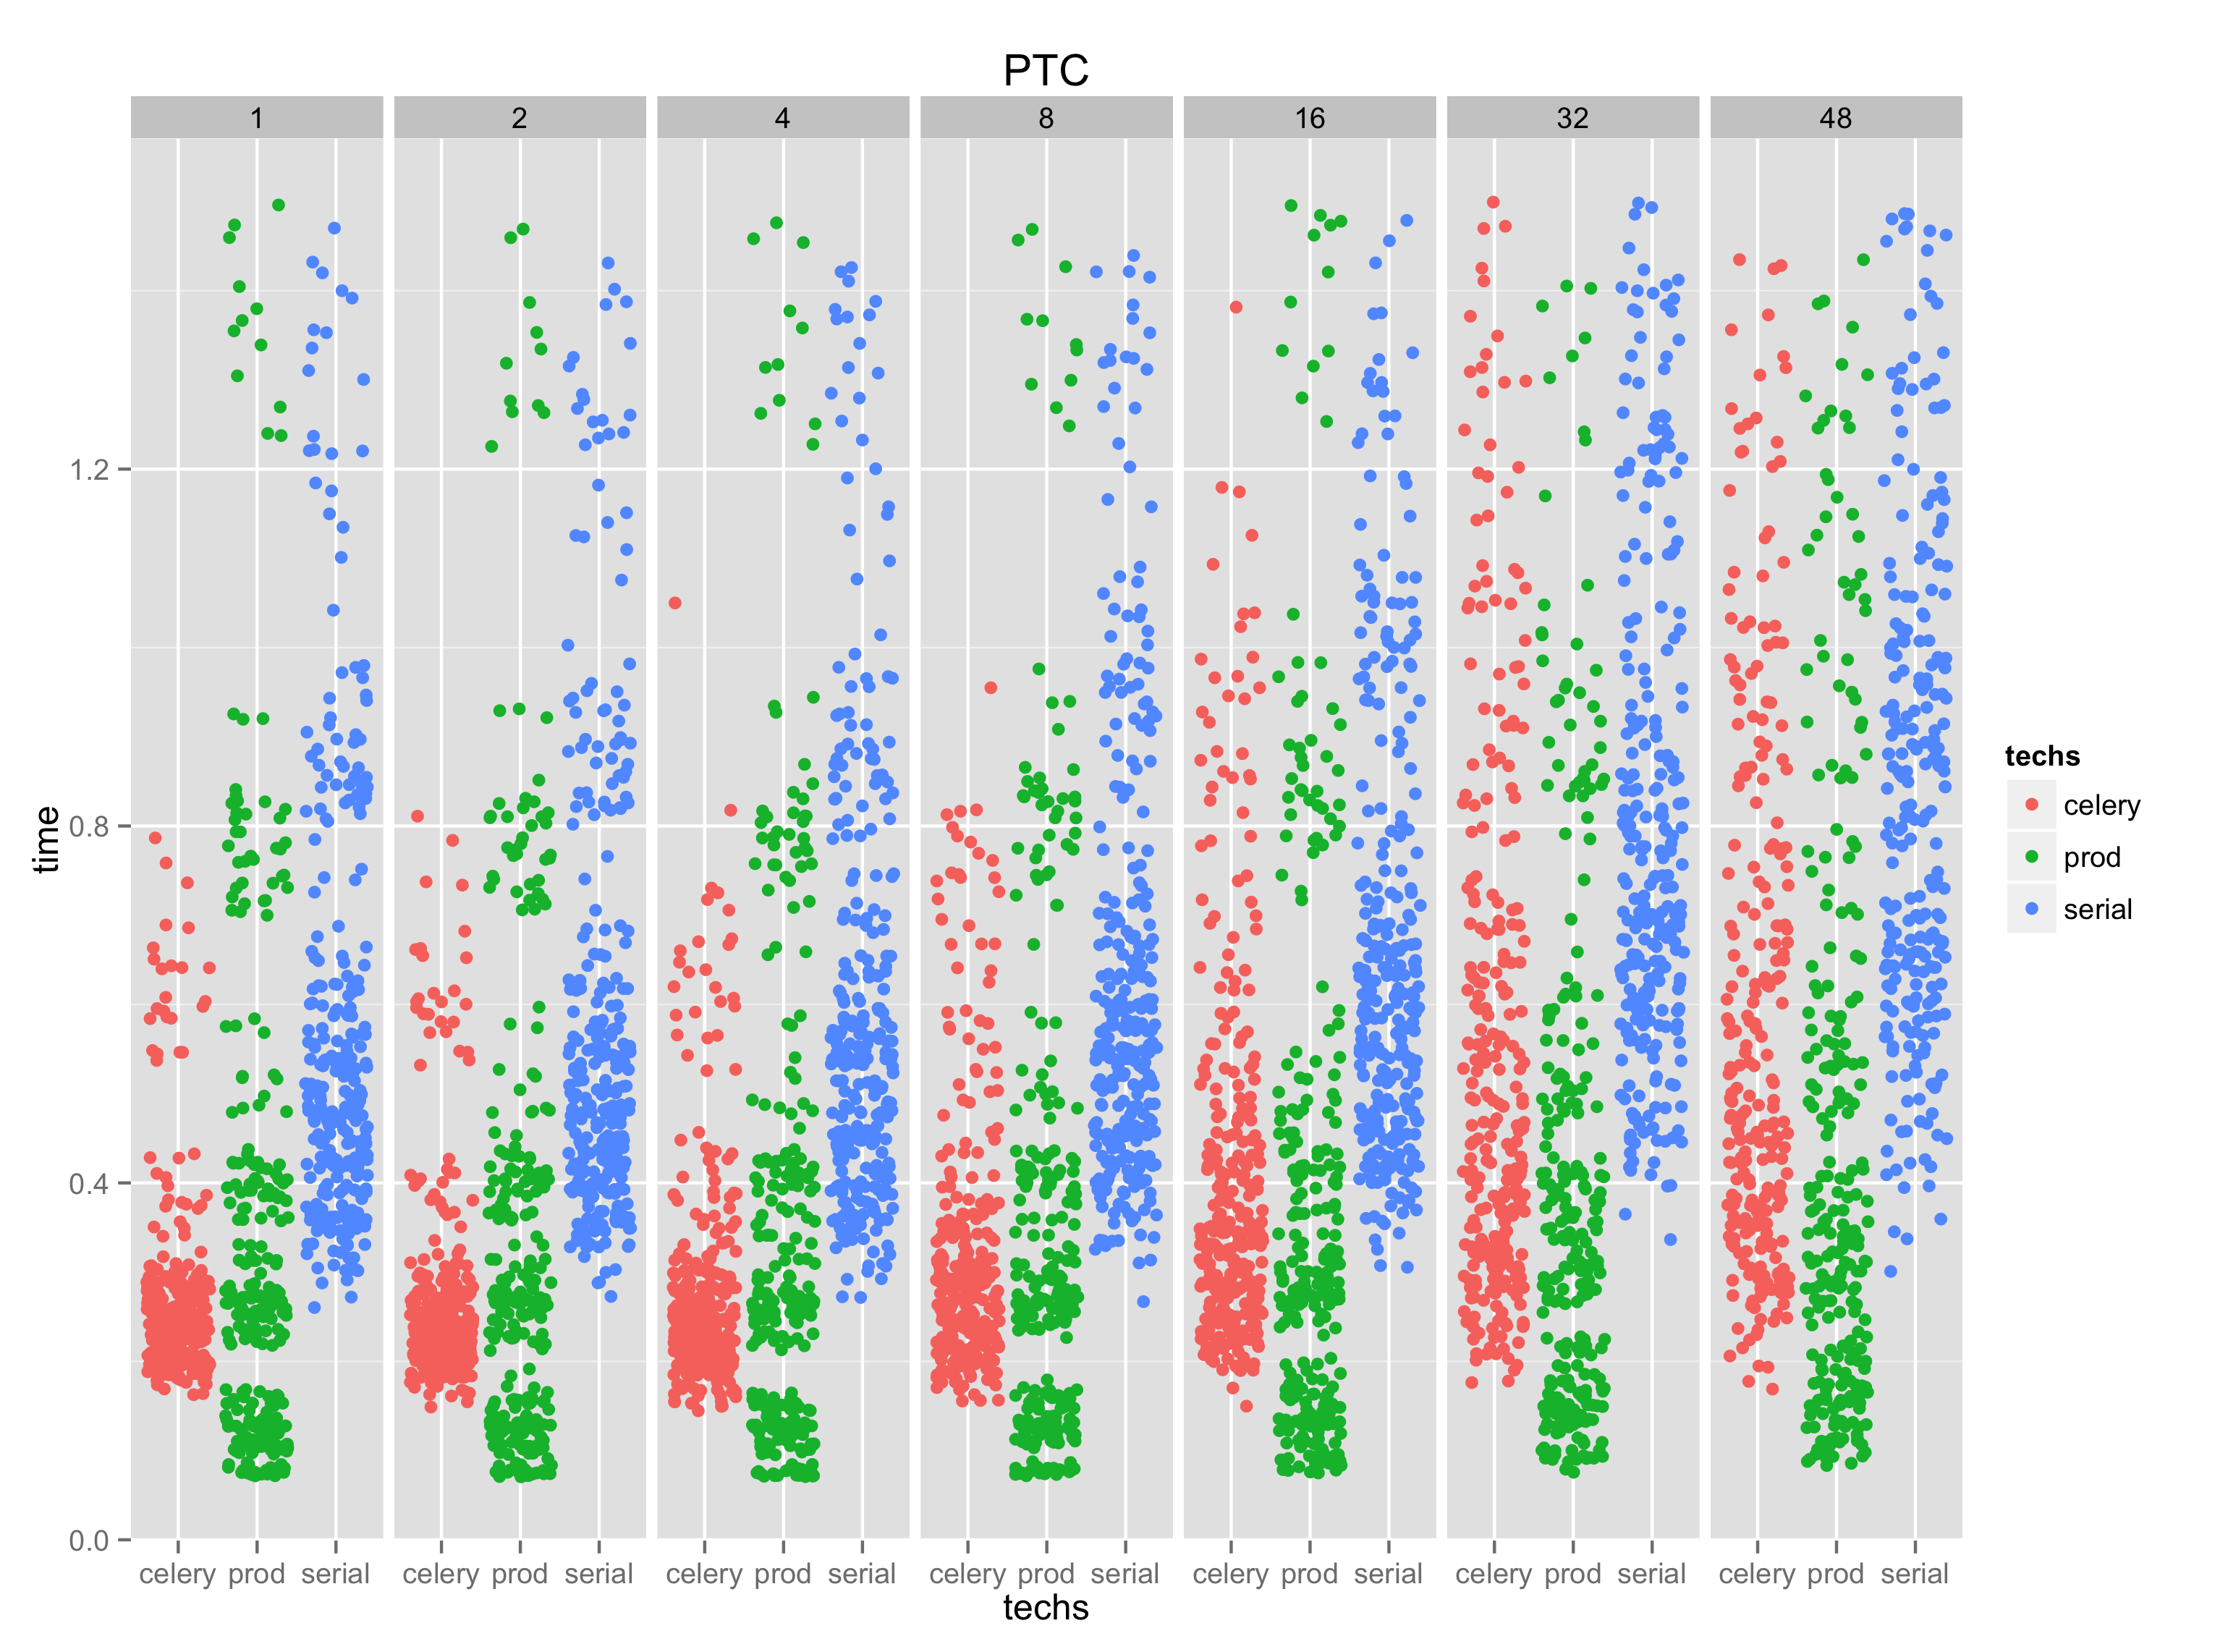
\includegraphics[width=\linewidth]{images/PTC.png}
\end{figure}
\end{frame}

\begin{frame}
\begin{figure}
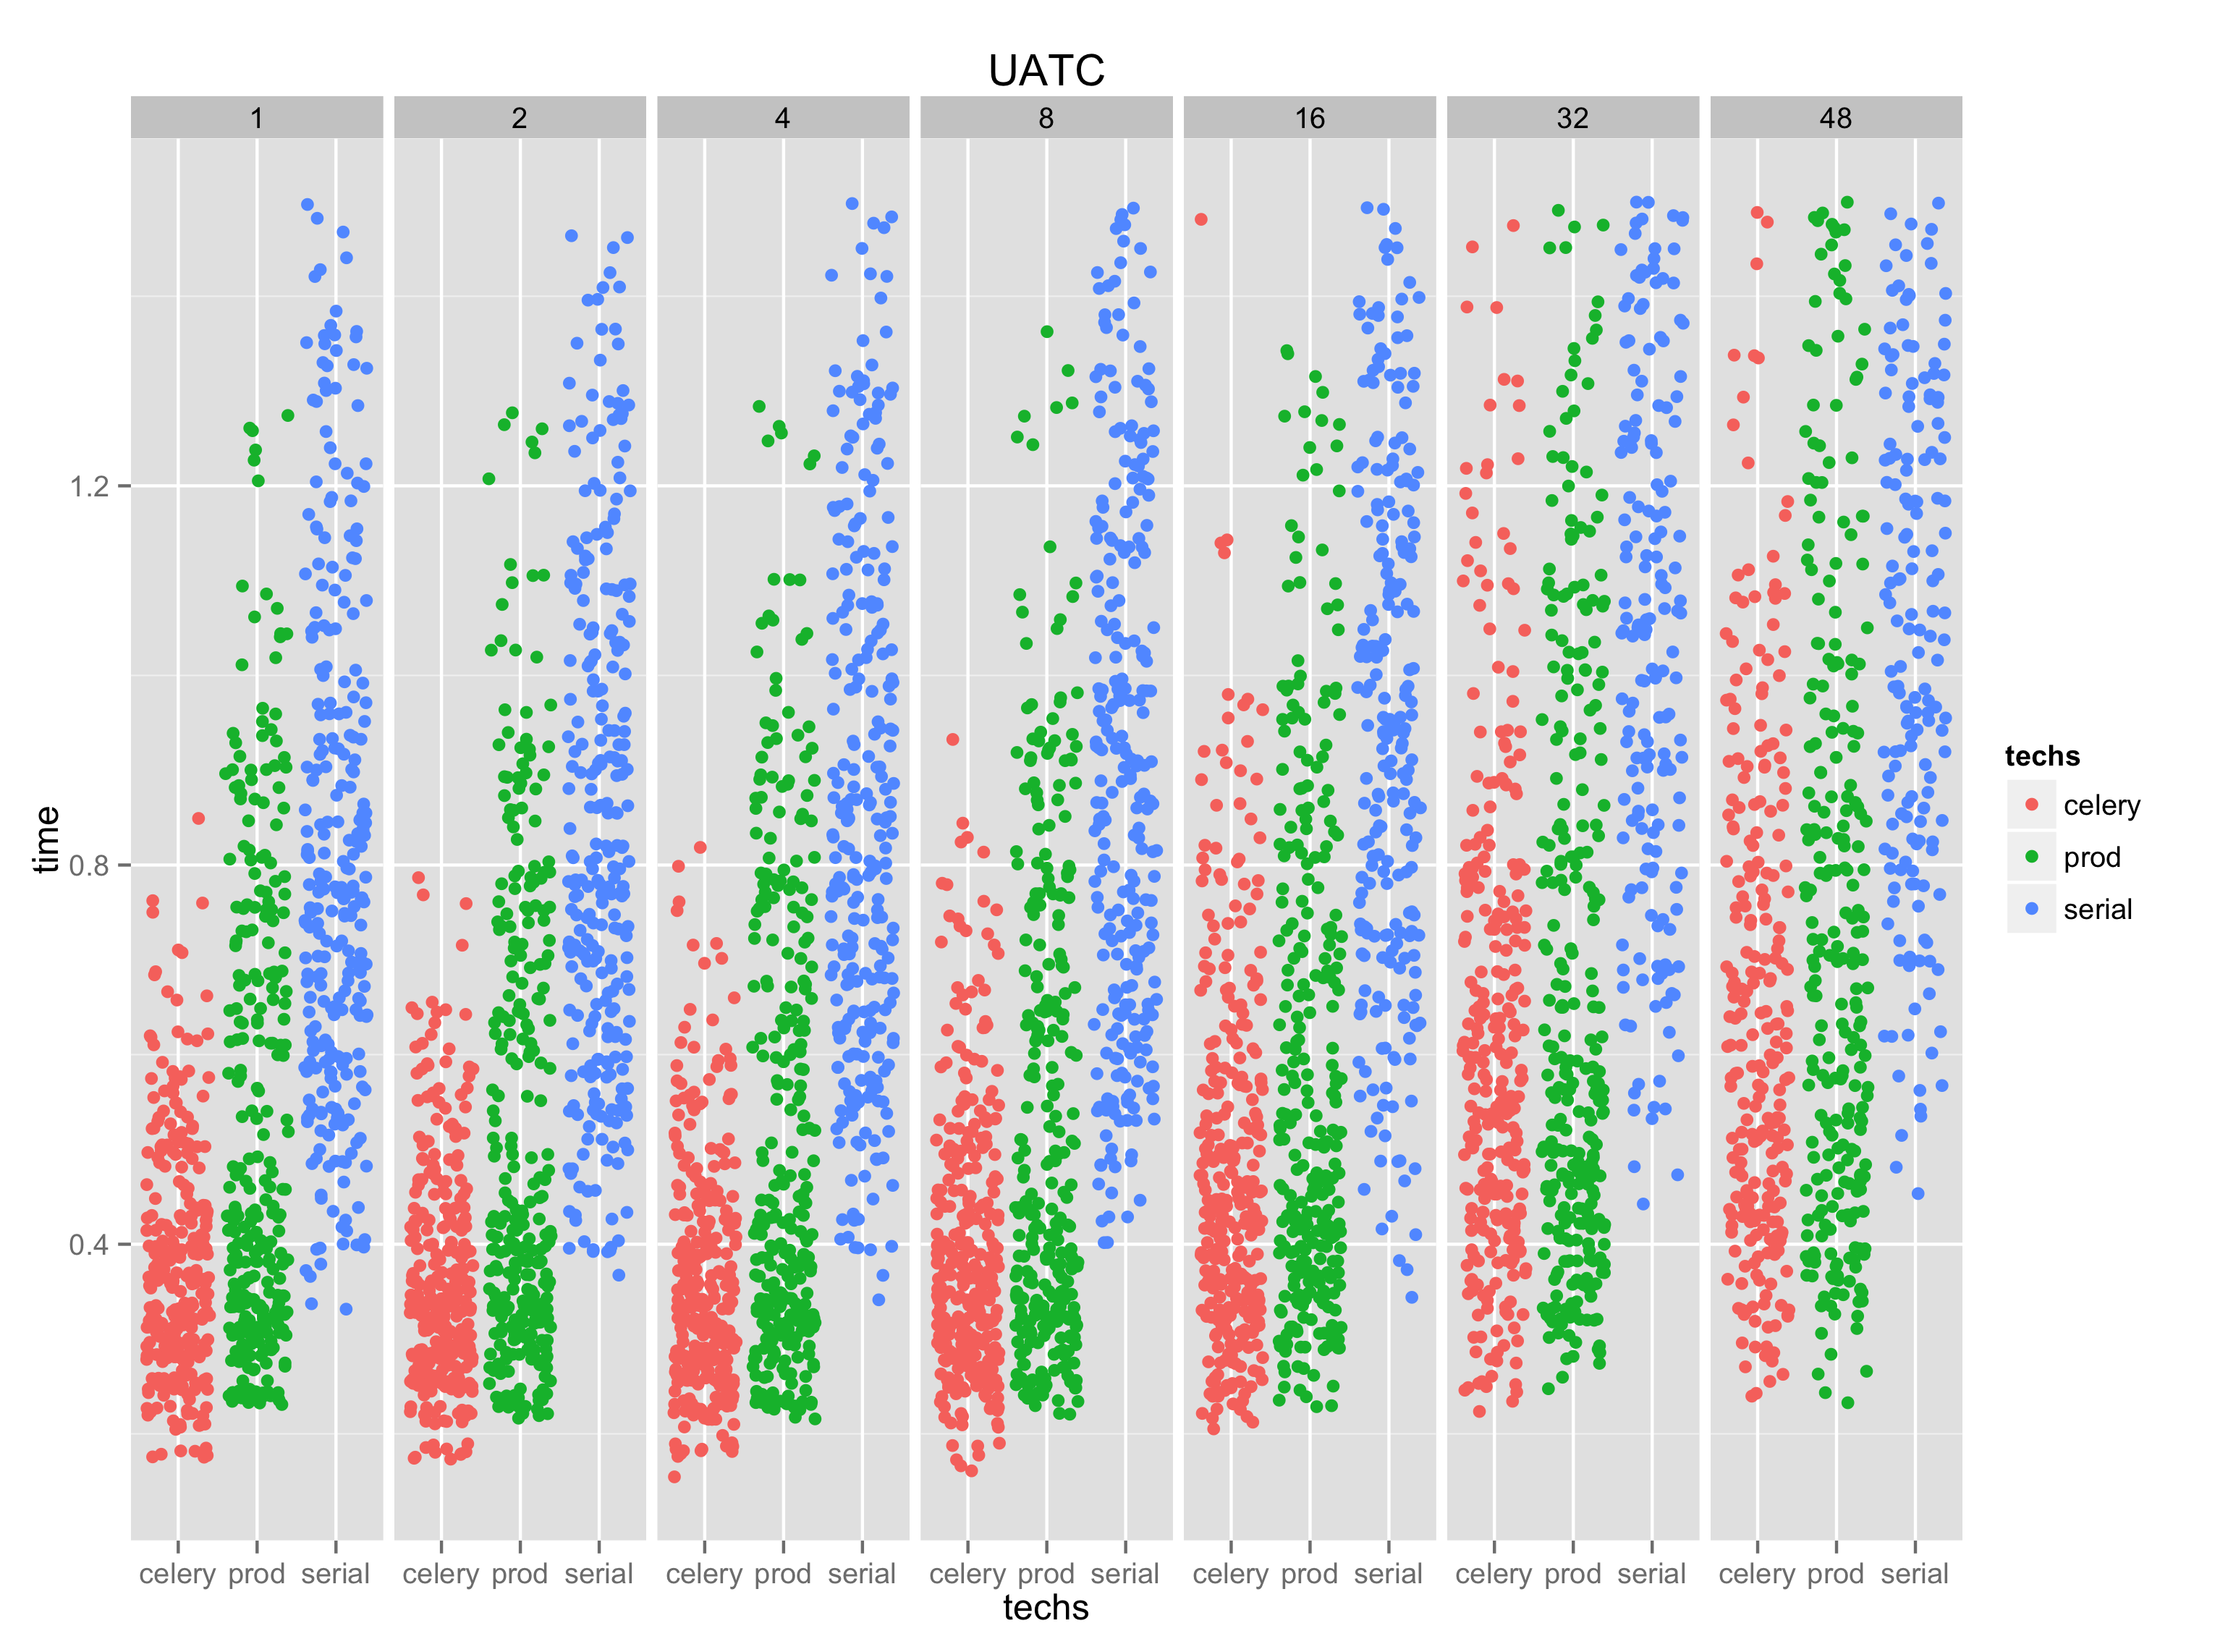
\includegraphics[width=\linewidth]{images/UATC.png}
\end{figure}
\end{frame}

\begin{frame}
\frametitle{Summary}
\begin{itemize}
\item ACB/PCB: comparing with production and serial in ec2,  celery speedup performance very much, also celery/rabbitmq is more stable.
\item AH/PH: celery/rabbitmq is more stable, specially for big data range, performance hierarchies disappeared in celery's graphics.
\item ATC/PTC/UATC: celery has better performance and also more stabler than production and serial one.
\end{itemize}
\end{frame}

\begin{frame}
\frametitle{Is it necessary parallelize AH/PU?}
\begin{itemize}
\item although serial AH/PH has good performance for small date range, parallelized AH/PU is more stabler than serial one.
\item it's more manageable if we parallelize AH/PH, that all feature will be follow same architecture and computing flow.
\end{itemize}
\begin{figure}
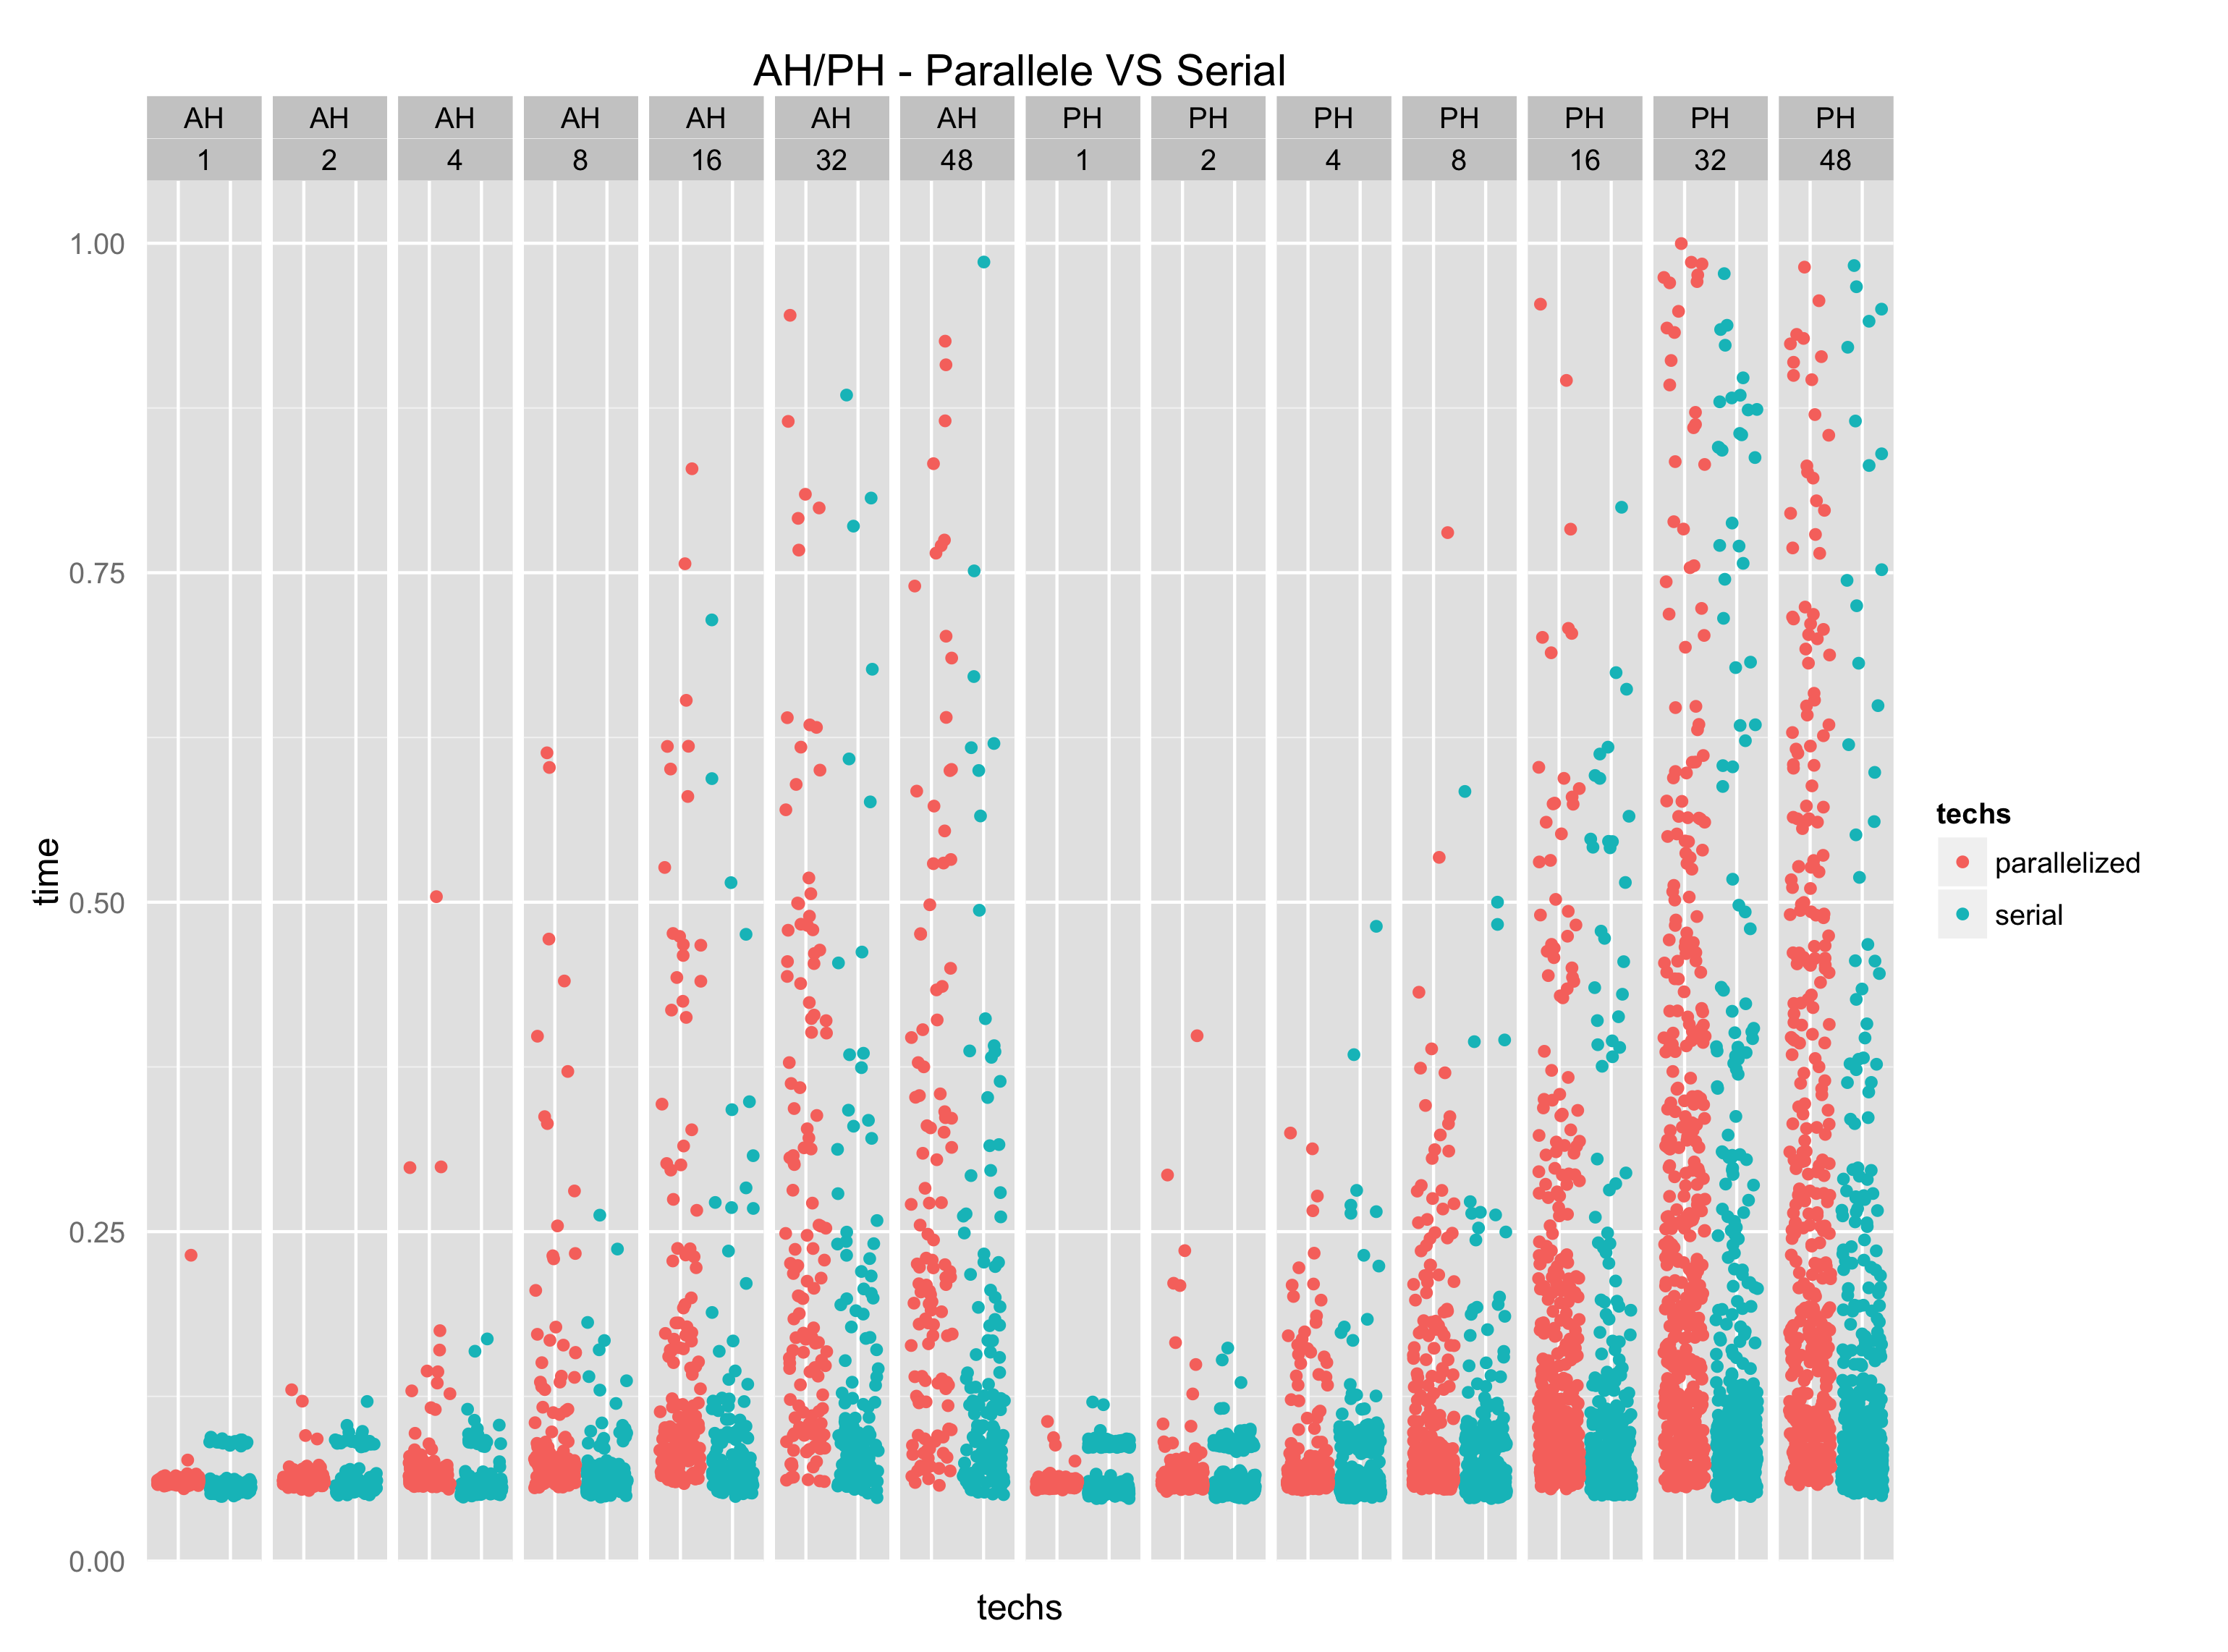
\includegraphics[width=10cm,height=6cm]{images/ah_ph_parallel_vs_serial.png}
\end{figure}
\end{frame}

%------------------------------------------------
\begin{frame}
\Huge{\centerline{The End}}
\end{frame}

%----------------------------------------------------------------------------------------
\end{document} 
